%%%%%%%%%%%%%%%%%%%%%%%%%%%%%%%%%%%%%%%%%%%%%%%%%%%%%%%%
%                       Assignment 2                   %
%                                                      %
% Author: Michael P. J. Camilleri					   %
%                                                      %
% Based on the Cleese Assignment Template for Students %
% from http://www.LaTeXTemplates.com.				   %
%                                                      %
% Original Author: Vel (vel@LaTeXTemplates.com)		   %
%													   %
% License:											   %
% CC BY-NC-SA 3.0 									   %
% (http://creativecommons.org/licenses/by-nc-sa/3.0/)  %
% 													   %
%%%%%%%%%%%%%%%%%%%%%%%%%%%%%%%%%%%%%%%%%%%%%%%%%%%%%%%%

%--------------------------------------------------------
%   IMPORTANT: Do not touch anything in this part
\documentclass[12pt]{article}
\input{style.tex}



% Options for Formatting Output

\global\setbool{clearon}{true} %
\global\setbool{authoron}{true} %



\newcommand{\assignmentQuestionName}{Question}
\newcommand{\assignmentTitle}{Assignment\ \#2}

\newcommand{\assignmentClass}{IAML -- INFR10069 (LEVEL 10)}

\newcommand{\assignmentWarning}{NO LATE SUBMISSIONS} % 
\newcommand{\assignmentDueDate}{Friday,\ November\ 15,\ 2019 @ 16:00}
%--------------------------------------------------------

%--------------------------------------------------------
%   IMPORTANT: Specify your Student ID below [You will need to uncomment the line, else compilation will fail]. Make sure to specify your student ID correctly, otherwise we may not be able to identify your work and you will be marked as missing.
%\newcommand{\assignmentAuthorName}{s6666666}
%--------------------------------------------------------

\begin{document}
\maketitle
\thispagestyle{empty}



%%%%%%%%%%%%%%%%%%%%%%%%%%%%%%%%%%%%%%%%%%%%%%%%%%%%%%%%%%%%%%%%%%%%%%%%%%%%%%
%============================================================================%
%%%%%%%%%%%%%%%%%%%%%%%%%%%%%%%%%%%%%%%%%%%%%%%%%%%%%%%%%%%%%%%%%%%%%%%%%%%%%%


\assignmentSection{Part A: 20-NewsGroups [60 Points]}




\begin{question}{(10 points) Exploratory Analysis}

\questiontext{We will begin by exploring the Dataset to get some insight about it.}



\begin{subquestion}{(5 points) Focusing first on the training set, summarise the key features/observations in the data: focus on the dimensionality, data ranges, feature and class distribution and report anything out of the ordinary. What are the typical values of the features like?}


\answerbox{12em}{
From the columns in the train set, we can see that every feature is a word's term frequency value in a sample, so all the values of features will be in [0,1] and typical value will be 0.  \\
The train set has 5648 samples and 1001 columns. What's more, it has 1000 features and 1 label. As for label, there has 8 classes and 7 classes' number is about 740 while class 7 only have 471 samples. However, some samples only have a 1 without any values is not 0 which means the sample only have one word. That's strange.
}



\end{subquestion}


\begin{subquestion}{(3 points) Looking now at the Testing set, how does it compare with the Training Set (in terms of sizes and feature-distributions) and what could be the repurcussions of this?}


\answerbox{10em}{
By loading the test set we can see that the test set has 1883 and 1001 columns. The test set has the same features as train set and test set's feature data ranges and distributions. As for label, there also has 8 classes and 7 classes' number is about 240 while class 7 only have 157 samples. This represents that the test set has the same distribution with train set and we can predict test set effectively by learning train set.
}



\end{subquestion}

\begin{subquestion}{(2 points) Why do you think it is useful to consider TF-IDF weights as opposed to just the frequency of times a word appears in a document as a feature?}



\answerbox{10em}{
When we just use the frequency of times a word appears in a document as a feature, there is a problem: some word like "is" will have a high frequency but they don't distinguish the document from others because other documents will have high values for these words too. So, we must decrease the influence of these words and take idf into account. If a word is common, it will appear in many documents thus has a low idf value. So the tf-idf value will be low too and it will not has big influence on our performance.
}



\end{subquestion}



\end{question}


%============================================================================%

\begin{question}{\label{Q_UNSUP_LEARN}(24 points) Unsupervised Learning}

\questiontext{We will now explore the documents in some detail by way of clustering.}



\begin{subquestion}{(2 points) The K-Means algorithm is non-deterministic. Explain why this is, and how the final model is selected in the SKLearn implementation of \href{https://scikit-learn.org/stable/modules/clustering.html}{KMeans}.}



\answerbox{8em}{
Because kMeans must choose k centroids, and different initialization of centroids will affect the performance. So it is highly dependent on the initialization of the centroids. \\
As a result, the algorithm is often done several times with different initialization of the centroids. What's more, scikit-learn implement a k-means++ initial scheme to initialize the centroids to be (generally) distant from each other.
}



\end{subquestion}


\begin{subquestion}{(1 point) One of the parameters we need to specify when using k-means is the number of clusters. What is a reasonable number for this problem and why?}



\answerbox{5em}{
In my opinion, the number is 8. There are only 8 classes and choosing the number of clusters as 8 may cluster the data appropriately.
}



\end{subquestion}


\begin{subquestion}{(5 points) We will use the Adjusted Mutual Information (AMI) \ie \href{https://scikit-learn.org/stable/modules/clustering.html\#mutual-info-score}{\texttt{adjusted\_mutual\\\_info\_score}} between the clusters and the true (known) labels to quantify the performance of the clustering. Give an expression for the MI in terms of entropy. In short, describe what the MI measures about two variables, why this is applicable here and why it might be difficult to use in practice. \hint{MI is sometimes referred to as Information Gain: note that you are asked only about the standard way we defined MI and not the AMI which is adjusted for the size of the domain and for chance agreement.}}



\answerbox{16em}{
1. MI can be expressed as $I(X;Y)=H(X)+H(Y)-H(X,Y)$, in which $H$ refer to entropy.  \\
2. Intuitively, mutual information measures the information that $X$ and $Y$ share: It measures how much knowing one of these variables reduces uncertainty about the other. So, it can measure similarity between two labels of the same data. \\
3. Because MI is independent of the absolute values of the labels:  a permutation of the class or cluster label values won’t change the score value in any way, so it can be used to evaluate cluster result. However, MI have some shortcomings: MI's max value isn't 1, which is therefore harder to judge; when prediction get independent labels, the MI will reach the max value too. But we have 1883 test data and only 8 classes, so we won't get independent labels and can use MI to evaluate.
}



\end{subquestion}

\begin{subquestion}{(4 points) Fit K-Means objects with \texttt{n\_clusters} ranging from 2 to 12. Set the random seed to 1000 and the number of initialisations to 50, but leave all other values at default. For each fit compute the adjusted mutual information (there is an SKLearn \href{https://scikit-learn.org/stable/modules/generated/sklearn.metrics.adjusted_mutual_info_score.html}{function} for that). Set \texttt{average\_method=`max'}. Plot the AMI scores against the number of clusters (as a line plot).}



\answerbox{40em}{
\begin{center}
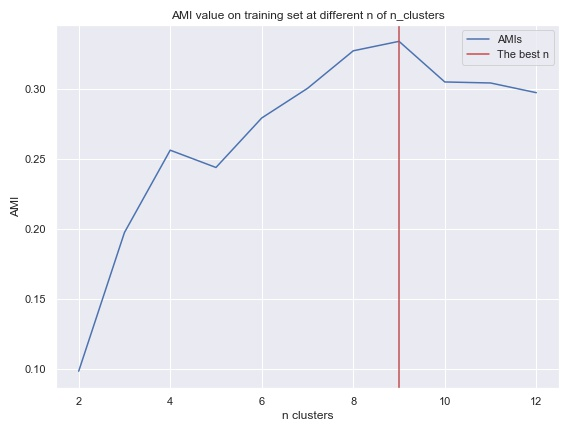
\includegraphics[width=1.0\textwidth] {Figure/Figure_7.jpg}
\end{center}
}



\end{subquestion}

\begin{subquestion}{\label{Q_CLUSTER_TRENDS}(3 points) Discuss any trends and interesting aspects which emerge from the plot. Does this follow from your expectations?}



\answerbox{10em}{
We can see that: as the number of n\_clusters increases, the AMI of cluster result increases too. However, when n\_clusters = 9, the AMI get the highest value. Then, AMI begins to decrease. \\
So, the result is very close to my expectation because my expectant number is 8. There only has a difference of 1.
}



\end{subquestion}

\begin{subquestion}{\label{Q_CLUSTER_FOUR}(6 points) Let us investigate the case with four (4) clusters in some more detail. Using seaborn's \href{https://seaborn.pydata.org/generated/seaborn.countplot.html}{\texttt{countplot}} function, plot a bar-chart of the number of data-points with a particular class (encoded by colour) assigned to each cluster centre (encoded by position on the plot's x-axis). As part of the cluster labels, include the total number of data-points assigned to that cluster.}



\answerbox{40em}{
\begin{center}
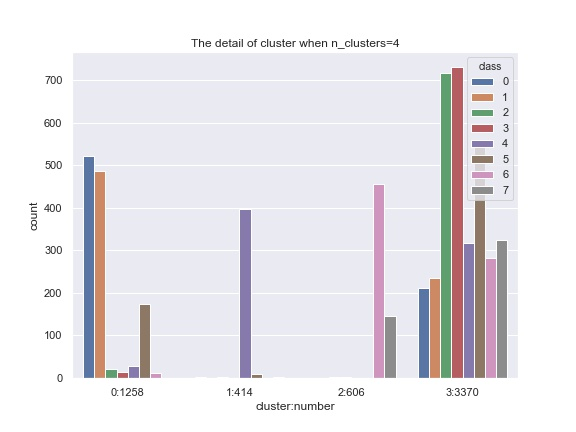
\includegraphics[width=1.0\textwidth] {Figure/Figure_8.jpg}
\end{center}
}



\end{subquestion}

\begin{subquestion}{(3 points) How does the clustering in Question\ref{Q_UNSUP_LEARN}:\ref{Q_CLUSTER_FOUR} align with the true class labels? Does it conform to your observations in Question\ref{Q_UNSUP_LEARN}:\ref{Q_CLUSTER_TRENDS}?}



\answerbox{14em}{
From the image we can see that: When the n\_clusters=4, the clustering result isn't good. 
For cluster 0, 1258 data-points are assigned to it. In which, the major data-points is from class 0 and 1. And data-points from 5 also have a significant proportion. 
For cluster 1 and 2, the cluster result is not bad. The major class of cluster 1 is class 4, and the major class of cluster 2 is class 6. \\
However, for cluster 3, the result is very disappointing. It contains data-points from all the classes and all the classes' data-points have a significant proportion. \\
So, the main problem is that the number of clusters is so small that KMeans algorithm can not find appropriate cluster for all the classes. Thus, increasing the number of n\_clusters may get better performance. Obviously, it conform the observations in Question\ref{Q_UNSUP_LEARN}:\ref{Q_CLUSTER_TRENDS}.
}



\end{subquestion}



\end{question}

%============================================================================%

\begin{question}{(26 points) Logistic Regression Classification}
\label{Q_LR_NG}
\questiontext{We will now try out supervised classification on this data. We will focus on Logistic Regression and measure performance in terms of the \href{https://scikit-learn.org/stable/modules/generated/sklearn.metrics.f1_score.html}{F1} score (familiarise yourself with this score which is related to the precision and recall scores that we learnt about in class).}



\begin{subquestion}{(3 points) What is the F1-score, and why is it preferable to accuracy in our problem? How does the macro-average work to extend the score to multi-class classification?}



\answerbox{8em}{
First give the expression of F1 score: $F1 = 2*\frac{P*R}{P+R}$, in which P is precision and R is recall. We can see that F1 score take both precision and recall into account. Only if precision and recall are high, F1 score can be a high value. So, using it is preferable to accuracy.   \\
As for macro-average method, it calculate metrics for each label, and find their unweighted mean. This does not take label imbalance into account.
}



\end{subquestion}


\begin{subquestion}{(2 points) As always we start with a simple baseline classifier. Define such a classifier (indicating why you chose it) and report its performance on the \textbf{Test} set. Use the `macro' average for the \texttt{f1\_score}.} %\hint{For the baseline, the classifier should use only the target labels.}



\answerbox{8em}{
To define a baseline model, I choose a random guess machine. Because without any prior knowledge of the dataset, what we can do is just do random guess. And with random guess, then we can see how much better our model do comparing to the case that we don't learn anything from dataset. So, the base line is $f(x)=R(class)$, in which R means random choosing. \\
So, the F1 score of baseline on testing set is 0.127, which is a bad performance.
}



\end{subquestion}

\begin{subquestion}{(3 points) We will now train a \href{https://scikit-learn.org/stable/modules/generated/sklearn.linear_model.LogisticRegression.html}{LogisticRegression} Classifier from SKLearn. By referring to the documentation, explain how the Logistic Regression model can be applied to classify multi-class labels as in our case. \hint{Limit your explanation to methods we discussed in the lectures.}}



\answerbox{9em}{
As we all known, Logistic Regression is a binary classification method. To solve a multi-class class, SKlearn uses the one-vs-rest (OvR) scheme. For every class in the task, there will be a classifier to classify whether a sample belongs to this class. Then, combine all the results for every class we can get a final multi-class classification result.
}



\end{subquestion}

\begin{subquestion}{(4 points) Train a Logistic Regressor on the training data. Set \texttt{solver=`lbfgs'}, \texttt{multi\_class=`multinomial'} and \texttt{random\_state=0}. Use the Cross-Validation object you created and report the average validation-set F1-score as well as the standard deviation. Comment on the result.}



\answerbox{9em}{
The average validation-set F1-score is 0.669. \\
The standard deviation of validation-set F1-score is 0.017. \\
So, we can see that though Logistic Regression is a simple model, it can learn knowledge from dataset and do much better than random guess.
}



\end{subquestion}

\begin{subquestion}{\label{Q_LOG_REG_PLT}(5 points) We will now optimise the Regularisation parameter $C$ using cross-validation. Train a logistic regressor for different values of $C$: in each case, evaluate the F1 score on the training and validation portion of the fold. That is, for each value of $C$ you must provide the training set and validation-set scores per fold and then compute (and store) the average of both over all folds. Finally plot the (average) training and validation-set scores as a function of $C$. \hint{Use a logarithmic scale for $C$, spanning 19 samples between $10^{-4}$ to $10^5$.}}



\answerbox{40em}{
\begin{center}
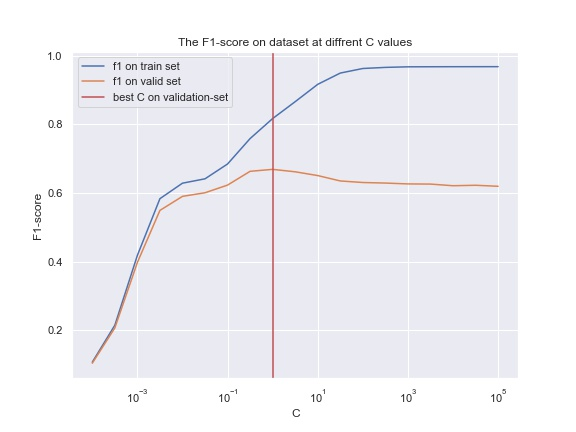
\includegraphics[width=1.0\textwidth] {Figure/Figure_9.jpg}
\end{center}
}



\end{subquestion}

\begin{subquestion}{(7 points) What is the optimal value of $C$ (and the corresponding score)? How did you choose this value? By making reference to the effect of the regularisation parameter $C$ on the optimisation, explain what is happening in your plot from Question \ref{Q_LR_NG}:\ref{Q_LOG_REG_PLT} \hint{Refer to the documentation for $C$ in the \href{https://scikit-learn.org/stable/modules/generated/sklearn.linear_model.LogisticRegression.html}{LogisticRegression} page on SKLearn}.}



\answerbox{11em}{
The optimal C value is 1 which is chose by performance on validation set. When C=1, the average F1-score on training set is 0.817, and it's 0.669 on validation set.   \\
Actually, the C is inverse of regularization strength. So, when C is small, the Logistic Model must be very simple and can not learn enough knowledge from dataset and perform bad on both two sets. Thus, increasing C make model do better. However, when C is too big that model can learn complicated function from training set which is not  appropriate for validation set. Thus, the model will do perfect on training set while performance on validation set will worse than it on training set.
}



\end{subquestion}

\begin{subquestion}{(2 points) Finally, report the score of the best model on the test-set, after retraining on the entire training set (that is drop the folds). \hint{You may need to set \texttt{max\_iter = 200}.} Comment briefly on the result.}



\answerbox{7em}{
The F1-score on test-set of best model is 0.675. And the best model's F1-score on validation set is 0.669. So, the F1-scores is very close which shows that the parameters we set make the model have a low variance and have strong generalization ability.
}



\end{subquestion}


\end{question}




%============================================================================%




%%%%%%%%%%%%%%%%%%%%%%%%%%%%%%%%%%%%%%%%%%%%%%%%%%%%%%%%%%%%%%%%%%%%%%%%%%%%%%
%============================================================================%
%%%%%%%%%%%%%%%%%%%%%%%%%%%%%%%%%%%%%%%%%%%%%%%%%%%%%%%%%%%%%%%%%%%%%%%%%%%%%%

\clearpage

\assignmentSection{Part B: Bristol Air-Quality [90 points]}




\begin{question}{\label{Q_EXPLORATORY}(30 Points) Exploratory Analysis}

\questiontext{We will begin by exploring the Dataset to familiarise ourselves with it.}



\begin{subquestion}{(6 points) Summarise the key features/observations in the data: describe the purpose of each column and report (briefly) also on the dimensionality/ranges (ballpark figures only, and how they compare across features) and number of sites, and identify anything out of the ordinary/problematic: \ie look out for missing data and negative values. Why are the latter unreasonable in such a dataset? \hint{Refer to the documentation for how to interpret the pollutant values.}}



\answerbox{13em}{
After read the csv, we can get that there are 18 site and every record have 3 main features: NOx, NO and NO2. And the total number of records is 1306758.  
Then we can see that the info about NOx, which represents the together as oxides of nitrogen. The NOx feature has 1191220 records, the other is null. And there also has 85 negative values which may represent some errors. From the histogram of this feature, the main range of NOx is from zero to 1000. The NO2 feature has 1188426 records and 98 negative values.And the main range of NO2 feature is from zero to 200. The NO feature has 1197536 records and 542 negative values. main range is from 0 to 600. 
}



\end{subquestion}

\begin{subquestion}{(6 points) Repeat the same analysis but this time on a per-site basis. Provide a table with the number of samples and percentage of problematic samples (negative and missing) in each site. To report numbers, count a row which has at least one missing entry
as having missing data, and similarly for negative entries. \hint{Pandas has a handy method, \texttt{to\_latex()}, for generating a latex table from a dataframe.}}



\answerbox{17em}{
\begin{tabular}{rrrrrrrr}
\toprule
 SiteID &   Count &  Negative &   Missing & SiteID &   Count &  Negative &   Missing \\
\midrule
      0 &    6446 &  0.000000 &  0.016134 &  9 &   22071 &  0.000000 &  0.053011 \\
      1 &  163111 &  0.000000 &  0.062902 & 10 &   96407 &  0.000041 &  0.035900 \\
      2 &   62990 &  0.000048 &  0.043483 & 11 &   20693 &  0.000870 &  0.019040 \\
      3 &   25464 &  0.007776 &  0.773327 & 12 &   45240 &  0.000000 &  0.174845 \\
      4 &   74787 &  0.000053 &  0.020685 & 13 &   12423 &  0.000161 &  0.514610 \\
      5 &  113952 &  0.000000 &  0.088283 & 14 &  113951 &  0.000000 &  0.105317 \\
      6 &  142141 &  0.000028 &  0.074440 & 15 &    2712 &  0.000000 &  1.000000 \\
      7 &  115162 &  0.002779 &  0.041950 & 16 &  154331 &  0.000136 &  0.065308 \\
      8 &   43824 &  0.000000 &  0.210570 & 17 &   91053 &  0.000022 &  0.062711 \\
\bottomrule
\end{tabular}
}



\end{subquestion}

\begin{subquestion}{(4 points) Briefly summarise how the sites compare in terms of number of samples and amount of problematic samples.}



\answerbox{11em}{
It's obvious that the negative values' percentage is very low from the question 4.1. And from the table in Question 4.2, we can see that the numbers of records at different sites range from 2712 to 163111. So, the records on different site have significant number differences. What's more, almost sites' records has a low percentage of missing values. However, at site 3, 13 and 15, there are 0.773, 0.515 and 1.000 respectively. So, these sites' records have less information.
}



\end{subquestion}

\begin{subquestion}{(3 points) Given that the columns are all oxides of nitrogen and hence we expect them to be related, we will now look at correlations in our data. This will also be useful in determining how well we can predict any one of the readings from the other two. Remove the data from sites 3 and 15 and compute the \textbf{Pearson} correlation coefficient between each of the three pollutant columns on the remaining data. Visualise the coefficients between each pair of columns in a table.}



\answerbox{10em}{
\begin{tabular}{lrrr}
\toprule
{} &   NOx &   NO2 &    NO \\
\midrule
NOx & 1.000 & 0.878 & 0.988 \\
NO2 & 0.878 & 1.000 & 0.808 \\
NO  & 0.988 & 0.808 & 1.000 \\
\bottomrule
\end{tabular}
}



\end{subquestion}

\begin{subquestion}{(2 points) Comment on the level of correlation between each pair of pollutants.}



\answerbox{7em}{
First, we can see that the correlation coefficient of NOx and NO2 is 0.878. However, the coefficient of NOx and NO is 0.988. Actually, from the main range of feature we can explain: the range of NO is larger than the range of NO2, so NO's value contributes more to NOx.
Second, the coefficient of NO and NO2 is 0.808, which show that NO and NO2 is related, but is not as strong as NOx with NO2 or NO.
}



\end{subquestion}



\begin{subquestion}{\label{CORRELATIONS}(5 points) For each of the three pollutants, compute the Pearson correlation between sites. \hint{You will need to remove the `Date Time' column and then group by the first level of the columns.} Then plot these as three heatmaps: show the values within the figures. \hint{Use the method \texttt{plot\_matrix()} from \texttt{mpctools.extensions.mplext}.}}



\answerbox{40em}{
\begin{center}
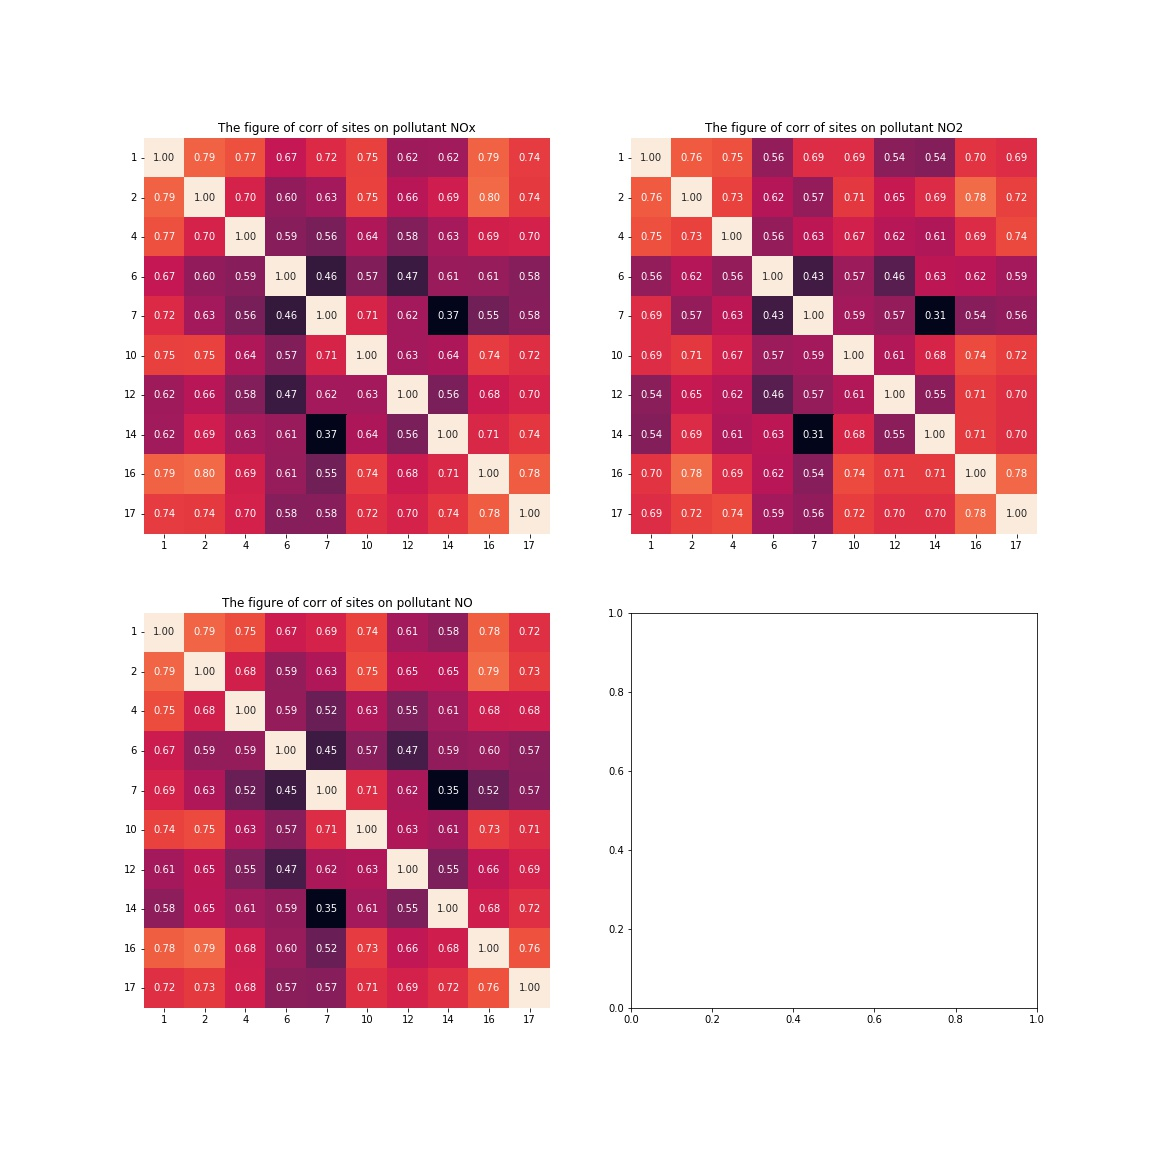
\includegraphics[width=1.0\textwidth] {Figure/Figure_1.jpg}
\end{center}
}



\end{subquestion}

\begin{subquestion}{(4 points) Comment briefly on your observations from Question \ref{Q_EXPLORATORY}:\ref{CORRELATIONS}: start by summarising the results from the NO gas and then comment on whether the same is observed in the other gases or if there is something different.}



\answerbox{12em}{
First, we observe the heat-map of the NO gas. So, site 1, 2, 10, 16 and 17 have several high Pearson correlation coefficient (>=0.7) with other site. Maybe they are site which are in the middle location. What's more, site 6, 7, 12 and 14 nearly have no related site. And pair of site 7 and 14 has the lowest coefficient which is 0.35.\\
Then, we can see that the same rule can be found in the other gases. To be exact, not the same, but very like.
}



\end{subquestion}

\end{question}


%============================================================================%

\begin{question}{(19 Points) Principal Component Analysis}

\questiontext{One aspect which we have not yet explored is the temporal nature of the data. That is, we need to keep in mind that the readings have a temporal aspect to them which can provide some interesting insight. We will explore this next.}



\begin{subquestion}{(1 point) Plot the first 5 lines of data (plot each row as a single line-plot).}



\answerbox{40em}{
\begin{center}
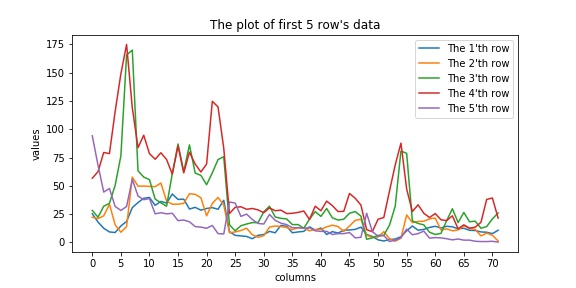
\includegraphics[width=1.0\textwidth] {Figure/Figure_2.jpg}
\end{center}
}



\end{subquestion}



\begin{subquestion}{(5 points) We will focus first on data solely from Site 1. Extract the data from this site, and run PCA with the number of components set to 72 for now. Set the \texttt{random\_state=0}. On a single graph plot: (i) the percentage of the variance explained by each principal component (as a bar-chart), (ii) the cumulative variance (line-plot) explained by the first $n$ components: (\hint{you should use \href{https://matplotlib.org/3.1.1/api/_as_gen/matplotlib.axes.Axes.twinx.html}{\texttt{twinx()}} to make the plot fit}), \textsl{and}, (iii) mark the point at which the number of components collectively explain at least 95\% of the variance (using a vertical line). \hint{Number components starting from 1.}}



\answerbox{40em}{
\begin{center}
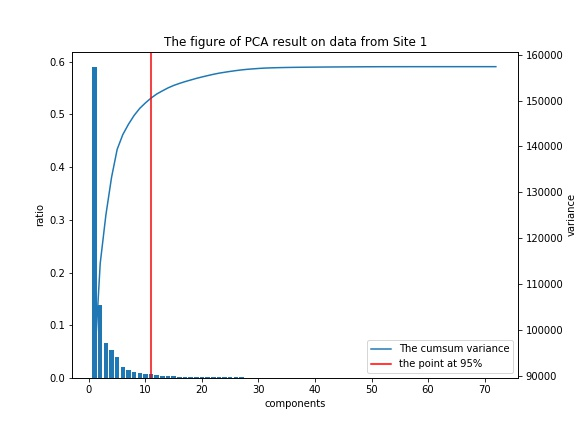
\includegraphics[width=1.0\textwidth] {Figure/Figure_3.jpg}
\end{center}
}



\end{subquestion}

\begin{subquestion}{(2 points) Interpret and summarise the above plot.}



\answerbox{9em}{
So, we have gotten the figure about PCA information and get some result:\\
1. The variance of first component is the largest, and it's ratio of the variance explained is 0.589; \\
2. First 10 components' sum value of variance explained exceeds 0.95, which means that the first 10 components have the nearly all of the information.\\
3. The components after serial number 30 have very low variance.
}



\end{subquestion}


\begin{subquestion}{(5 points) Generate three figures, one for the mean and one for each of the first 2 principal components: in each, plot the mean/component as three lines, one for each pollutant throught one day cycle. \hint{You will need to reshape the components appropriately.}}



\answerbox{50em}{
\begin{center}
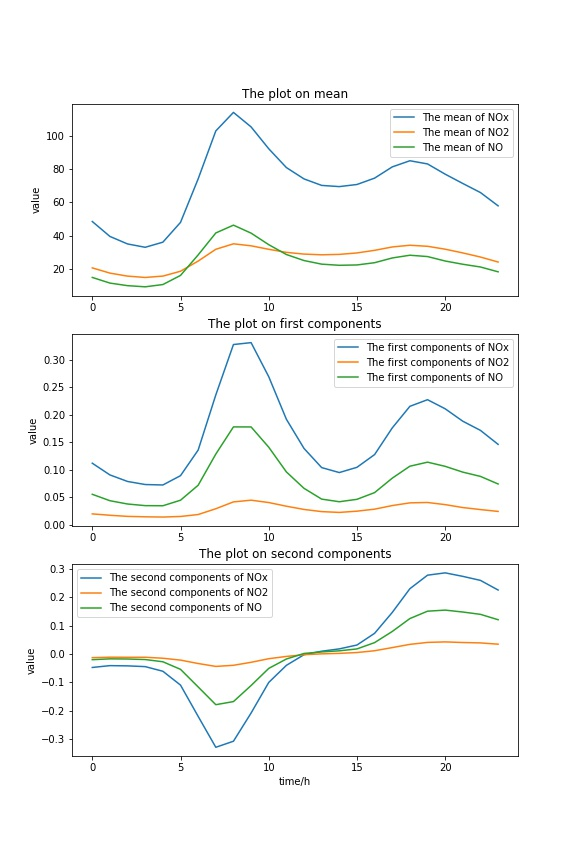
\includegraphics[width=0.9\textwidth] {Figure/Figure_4.jpg}
\end{center}
}



\end{subquestion}

\begin{subquestion}{(6 points) Focusing on the mean and first principal component, are there any significant patterns which emerge throughout the day? \hint{Think about car usage throughout the day.} What is different when interpreting the mean versus the first component? \hint{Do peaks signify the same thing in both cases?} Looking at the principal components only, are there any significant differences between the pollutants? Why could this be happening? \hint{You can refer to one of the limitations of PCA.}}



\answerbox{16em}{
Focus on the mean and first principal component, we can see that both of them have similar pattern. At 9 oclock and 18 oclock, there are peaks of NOx and NO both in mean and first principal component. It's obviously that it's related to the car usage throughout the day because at these times, car is highly used.\\
However, there also has some difference. In the mean's plot, the peak at 18 oclock is obvious, however, the peak at 18 oclock of the first component is not clear.\\
Then, we only talk about the principal components. However, the pattern between the components has a big difference. In the second principal component, a valley happened at 7 oclock while there is a peak at 8 oclock in first component. What's more, the peak at 18 oclock in the first principal component is delayed by about an hour in the second principal component. Maybe the original data is not highly linearly correlated, so PCA cannot performe well in second components.
}



\end{subquestion}

\end{question}

%============================================================================%


\begin{question}{\label{Q_LR_BA}(41 points) Regression}


\questiontext{Given our understanding of the correlation between signals and sites, we will now attempt to predict the NOx level for Site 17 given the value at the other sites. We will evaluate our models using the Root Mean Squared Error (RMSE) \ie the square root of the \href{https://scikit-learn.org/stable/modules/generated/sklearn.metrics.mean_squared_error.html}{mean\_squared\_error} score by sklearn.}



\begin{subquestion}{(2 points) First things first: since we are dealing with a supervised task, we will need to split our data into a training and testing set. Furthermore, since some of our regressors will involve hyper-parameter tuning, we will also need a validation set. Use the \texttt{multi\_way\_split()} method from \texttt{mpctools.extensions.skext} to split the data into a Training (60\%), Validation (15\%) and Testing (25\%) set: use the \href{https://scikit-learn.org/stable/modules/generated/sklearn.model_selection.ShuffleSplit.html}{ShuffleSplit} object from sklearn for the \texttt{splitter}. Set the random state to 0. \hint{The method gives you the indices of the split for each set, which can then be applied to multiple matrices.} Report the sizes of each dataset.}



\answerbox{4em}{
The size of training set is 8937.
The size of validation set is 2234.
The size of testing set is 3724.
}



\end{subquestion}

\begin{subquestion}{(4 points) Let us start with a baseline. By using only the $y$-values, what baseline regressor can you define (indicate what it does)? Implement it and report the RMSE on the training and validation sets. Interpret this relative to the statistics of the data.}



\answerbox{8em}{
Because of the only using of $y$-values, we can only define a baseline $f(y)=a$, $a$ is a constant. To find this constant, I use gradient descent method $a_j=a_{j-1}-\alpha\frac{1}{n}\sum_{i=1}^n 2*(a_{j-1}-y_i)$ to find the optimal a. The final result is $a=98.3206$, which is equal to the mean of the training set. \\
The RMSE on training set is 6354.30, while on validation set is 6432.84.
}



\end{subquestion}

\begin{subquestion}{(3 points) Let us now try a more interesting algorithm: specifically, we will start with \href{https://scikit-learn.org/stable/modules/generated/sklearn.linear_model.LinearRegression.html}{LinearRegression}. Train the regressor on the training data and report the RMSE on the training and validation set, and comment on the relative performance to the baseline.}



\answerbox{7em}{
The RMSE on training set is 1586.80.\\
The RMSE on validation set is 1691.46.\\
We can see that the result is much better than baseline because we have more feature and can get more parameters to learn.
}



\end{subquestion}



\begin{subquestion}{(5 points) We want to explore further what the model is learning. Explain why in Linear Regression, we cannot just blindly use the weights of the regression coefficients to evaluate the relative importance of each feature, but rather we have to normalise the features. By referring to the documentation for the \href{http://scikit-learn.org/stable/modules/generated/sklearn.linear_model.LinearRegression.html}{LinearRegression} implementation in SKLearn, explain what the normalisation does and how it helps in comparing features. Will this affect the performance of the Linear Regressor?}



\answerbox{10em}{
1. In Linear Regression, all the features may not in the same range. So, the weights cannot represent relative importance anytime. \\
2. The normalization transforms all features in the data to a specific range, so then  we can compare features. To normalise a feature, we subtract its mean and divide by its l2-norm. \\
3. No, it wont'. In Linear Regression, it is not sensitive to magnitude, the weights will keep the same because it is looking at proportional relationships.
}



\end{subquestion}

\begin{subquestion}{(5 points) Retrain the regressor, setting \texttt{normalize=True} and report (in a table) the ratio of the relative importance of each feature. Which is the most/least important site? How do they compare with the correlation coefficients for Site 17 as computed in Question \ref{Q_EXPLORATORY}:\ref{CORRELATIONS}, and why do you think that is?}



\answerbox{15em}{
The result table: \\
\begin{tabular}{rrrrrrrrr}
\toprule
     1 &      2 &      4 &       6 &      7 &     10 &     12 &     14 &     16 \\
\midrule
0.1156 & 0.0099 & 0.1341 & -0.0068 & 0.0594 & 0.0798 & 0.1291 & 0.0945 & 0.1618 \\
\bottomrule
\end{tabular}
\\
Site 16 is the most import site. Site 6 is the least import site. \\
This result is same as the correlation coefficients for Site 17. In Question \ref{Q_EXPLORATORY}:\ref{CORRELATIONS}, the correlation between site 16 and site 17 is the highest: 0.78, while it between site 6 and 17 is the lowest: 0.58. \\
So, we can get that in Linear Regression, if correlation coefficient for a feature and the label is higher, the feature will be more important. 
}



\end{subquestion}

\begin{subquestion}{(5 points) It might be that with non-linear models, we may get better performance. Let us try to use \href{https://scikit-learn.org/stable/modules/generated/sklearn.neighbors.KNeighborsRegressor.html}{K-Nearest-Neighbours}. Train a KNN regressor with default parameters on the training set and report performance on the training and validation set. \hint{it might be beneficial to set \texttt{n\_jobs=-1} to improve performance.} How does it compare with Linear Regression in terms of performance on both sets? What is a limitation of the KNN algorithm for our dataset?}



\answerbox{8em}{
The RMSE of kNN on training set is 1052.13.
The RMSE of kNN on validation set is 1624.67. \\
So, on training set, the result of KNN is much better than Linear Regression. While on validation set, the performance of KNN is very close to Linear Regression. Actually, KNN is a spatial algorithm while our dataset is not. So, KNN cannot find a generic function to do regression for our task.
}



\end{subquestion}

\begin{subquestion}{(4 points) The KNN regression allows setting a number of hyper-parameters. We will optimise only one: the number of neighbours to use. By using the validation set, find the optimal value for the \texttt{n\_neighbours} parameter out of the values [2, 4, 8, 16, 32]. Plot the training/validation RMSE and indicate (for example with a line) the best value for \texttt{n\_neighbours}.}



\answerbox{40em}{
\begin{center}
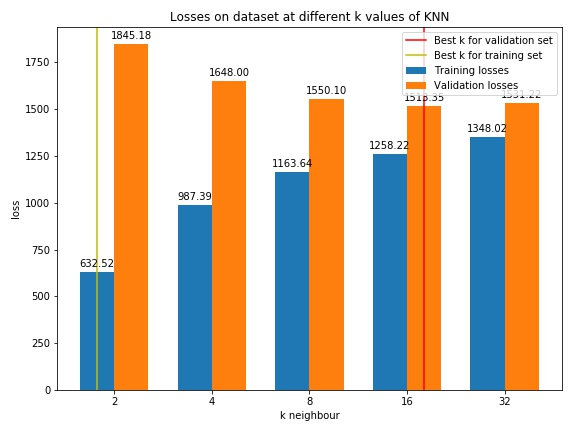
\includegraphics[width=1.0\textwidth] {Figure/Figure_5.jpg}
\end{center}
}



\end{subquestion}

\begin{subquestion}{(1 points) What is the best-case RMSE performance on the validation set for KNN?}



\answerbox{6em}{
From the image in Question 6:7, we can see that when k = 16, the KNN do best in validation set. And we can see when k increase, the generation ability of KNN is better.
}



\end{subquestion}

\begin{subquestion}{(4 points) Let us try one last regression algorithm: we will now use \href{https://scikit-learn.org/stable/modules/generated/sklearn.tree.DecisionTreeRegressor.html}{DecisionTreeRegressor}. Again, the algorithm contains a number of hyper-parameters, and we will optimise the depth of the tree. Train a series of Decision Tree Regressors, optimising (over the validation set) the \texttt{max\_depth} over the values [2, 4, 8, 16, 32, 64]. Set \texttt{random\_state=0}. Plot the training/validation RMSE and indicate (as before) the best value for \texttt{max\_depth}.}



\answerbox{40em}{
\begin{center}
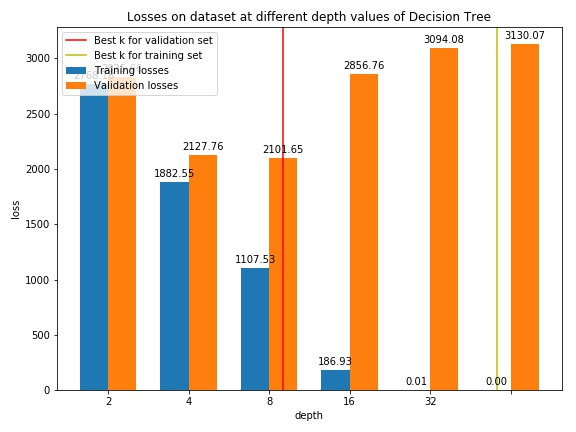
\includegraphics[width=1.0\textwidth] {Figure/Figure_6.jpg}
\end{center}
}



\end{subquestion}

\begin{subquestion}{(3 points) What is the best-case RMSE performance on the validation set? What do you notice from the plot about the performance of the Decision Tree Regressor?}



\answerbox{6em}{
When depth is 8, the Decision Tree do best on validation set. As the value of the depth increase, the Decision Tree do better on training set. when depth=32, the loss on training set is close to 0. However, the performance on validation set is getting better at first, then beginning to drop. 
}



\end{subquestion}

\begin{subquestion}{(5 points) To conclude let us now compare all the models on the testing set. Combine the training and validation sets and retrain the model from each family on it: in cases where we optimised hyper-parameters, set this to the best-case value. Report the testing-set performance of each model in a table \hint{You should have 4 values}.}



\answerbox{6em}{
The result of different models on testing set. \\
\begin{tabular}{lrrrr}
\toprule
{} &  Baseline &      LR &     KNN &      DT \\
\midrule
losses &   6369.91 & 1606.99 & 1264.59 & 1146.16 \\
\bottomrule
\end{tabular}
}



\end{subquestion}

\end{question}

%============================================================================


\end{document}
